\documentclass[journal,12pt,twocolumn]{IEEEtran}
\usepackage{graphicx}
\usepackage[margin=0.5in]{geometry}
\graphicspath{{./figs/}}{}
\usepackage{amsmath,amssymb,amsfonts,amsthm}
\newcommand{\myvec}[1]{\ensuremath{\begin{pmatrix}#1\end{pmatrix}}}
\usepackage{listings}
\usepackage{watermark}
\usepackage{titlesec}
\let\vec\mathbf
\lstset{
frame=single, 
breaklines=true,
columns=fullflexible
}
%\thiswatermark{\centering \put(0,-105.0){
\includegraphics[scale=0.5]{iith.png}} }

\title{\mytitle}
\title{
Matrix Assignment - Circle
}
\author{Adarsh Kumar (FWC22068)}
\begin{document}
\maketitle
\tableofcontents
\bigskip


\section{\textbf{Problem}}
The Circles ${x}^2$ + ${y}^2$ - 10x +16 = 0  and \hspace{5mm} ${x}^2$ + ${y}^2$ = ${r}^2$  intersect each other at two distinct points if .
\linebreak
A) $r<2$ \\ B) $r>8$\\ C) $2<r<8$ \\D) $2 \le r \le 8$
\section{\textbf{Solution}}

Given equation of circle 1 : $x^2+y^2-10x+16=0$\\
The standard equation of the conics is given as :
\begin{align}
\vec{x}^{\top}\vec{V}\vec{x}+2\vec{u}^{\top}\vec{x}+f=0
\end{align}
The given circle 1 can be expressed as conics with \\parameters
\begin{align}
	\vec{V} &= \vec{I}, \vec{u} = -\myvec{5 \\0}, f = 16
	\end{align}
	Radius and Centre are
\begin{align}
	r &=\sqrt{{\vec{u}^{\top}\vec{u}}-f },\\
	r &=\sqrt{25 -16} =3\\
	Center = \vec{A}=-u = (5,0)
    \end{align}
    Given equation of circle 2 : $x^2+y^2=r^2$\\
    The standard equation of the conics is given as :
\begin{align}
\vec{x}^{\top}\vec{V}\vec{x}+2\vec{u}^{\top}\vec{x}+f=0
\end{align}
The given circle 1 can be expressed as conics with \\parameters
\begin{align}
	\vec{V} &= \vec{I}, \vec{u} = -\myvec{0 \\0}, f = 0
	\end{align}
	Radius and Centre are
	\begin{align}
	r &=\sqrt{{\vec{u}^{\top}\vec{u}}-f },\\
	 Radius = r\\
	Center = \vec{A}=-u =  (0,0)  
	\end{align}

\section{\textbf{Conditions}}

Here we will vary the radius of circle 1 and one by one we will verify all the given options
\subsection{Conditon 1} When Radius r is less than 2 i.e $(r<2)$\\
here we have taken radius r = 1.5
\begin{figure}[h]
    \centering
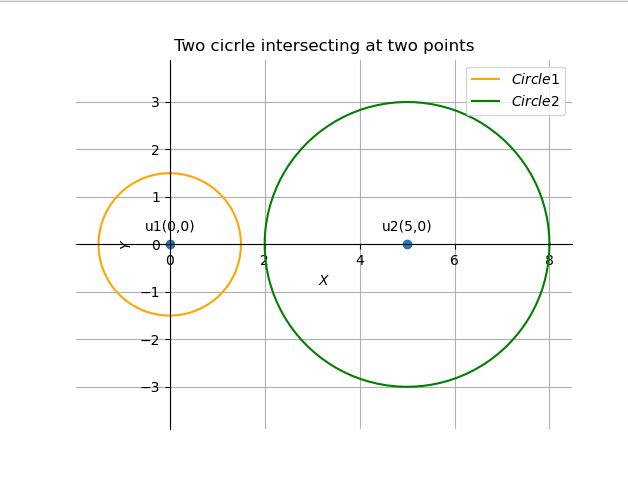
\includegraphics[width=\columnwidth]{circle1.png}
    \label{fig:my_label}
\end{figure}

By watching the above image , we can conclude that ,the  Circle 1 and Circle 2 will not intersect each other at any point when $r<2$ \\

\textbf{Conclusion 1} : option A is discarded as the Circle 1 and Circle 2 will not intersect each other at any point when $r<2$
\newpage
\subsection{Conditon 2} When Radius r is equal to 2 i.e $(r=2)$\\
here we have taken radius r = 2
\begin{figure}[h]
    \centering
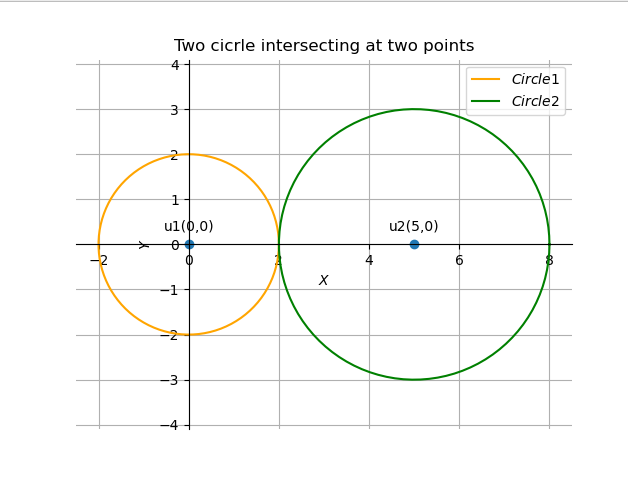
\includegraphics[width=\columnwidth]{circle2.png}
    \label{fig:my_label}
\end{figure}

By watching the above image , we can conclude that ,the  Circle 1 and Circle 2 will only touch each other but not intersect each other at any point when $r=2$ , So  option \textbf{D} is also discarded
\subsection{Conditon 3} When Radius r is greater than 2 i.e $(r>2)$\\
here we have taken radius r = 2.5
\begin{figure}[h]
    \centering
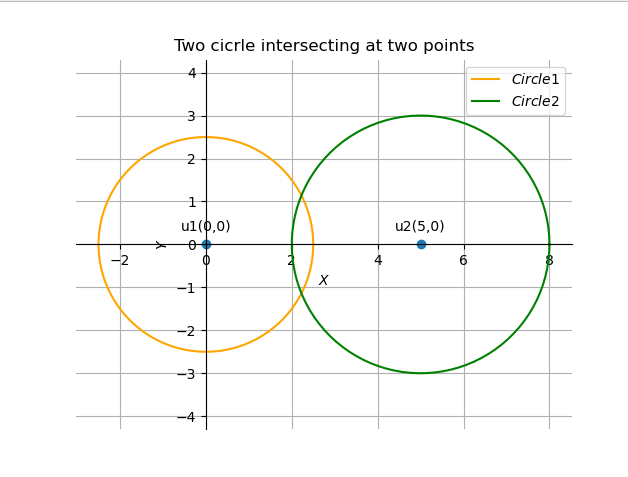
\includegraphics[width=\columnwidth]{circle3.png}
    \label{fig:my_label}
\end{figure}

By watching the above image , we can conclude that ,the  Circle 1 and Circle 2 will intersect each other at two point when $r>2$
\subsection{Conditon 4} When Radius r is less than 8 i.e $(r<8)$\\
here we have taken radius r = 7.5
\begin{figure}[h]
    \centering
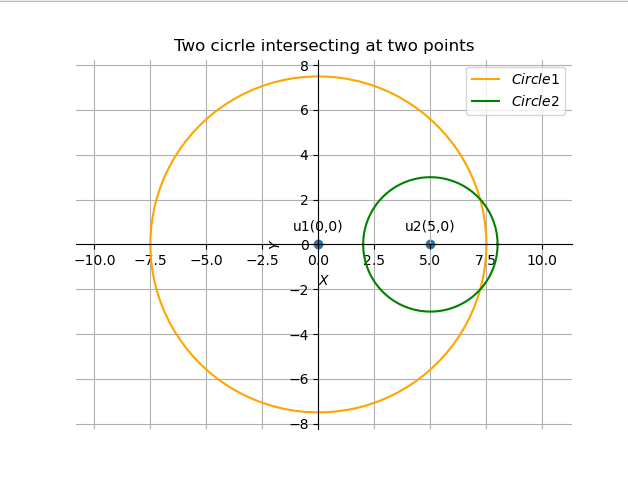
\includegraphics[width=\columnwidth]{circle4.png}
    \label{fig:my_label}
\end{figure}

By watching the above image , we can conclude that ,the  Circle 1 and Circle 2 will intersect each other at two point when $r<8$
\subsection{Conditon 5} When Radius r is equal to 8 i.e $(r=8)$\\
here we have taken radius r = 8
\begin{figure}[h]
    \centering
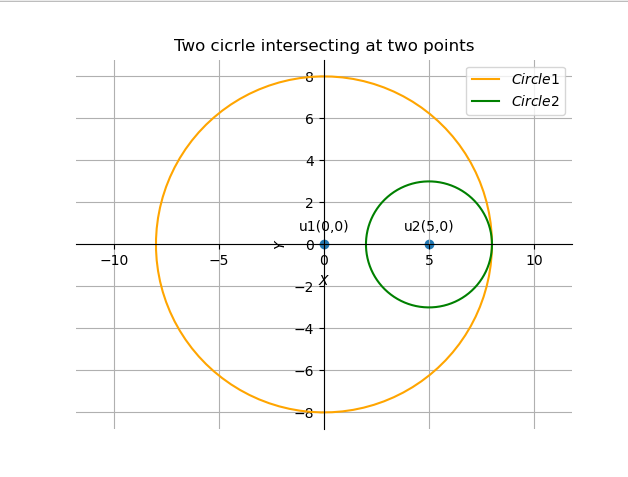
\includegraphics[width=\columnwidth]{circle5.png}
    \label{fig:my_label}
\end{figure}

By watching the above image , we can conclude that ,the  Circle 1 and Circle 2 will only touch each other but not intersect each other at any point when $r=8$ , So  option \textbf{D} is also discarded

\subsection{Conditon 6} When Radius r is greater than 8 i.e $(r>8)$\\
here we have taken radius r = 8.5
\begin{figure}[h]
    \centering
\includegraphics[width=\columnwidth]{circle6.png}
    \label{fig:my_label}
\end{figure}

By watching the above image , we can conclude that ,the  Circle 1 and Circle 2  will not intersect each other at any point when $r>8$ , So  option \textbf{B} is also discarded.
\\
\textbf{Finally we can conclude that the two circles will intersect at two points only if Radius r is between 2 and 8 i.e $ 2<r<8 $}
\\
\textbf{So we can conclude that option C is the only Correct answer to this problem}
\section{\textbf{Code Link}}

\begin{lstlisting}
https://github.com/aadrshptel/Fwc_module1/tree/main/Assignments/Matrix%20assignments/Circles/codes
\end{lstlisting}
Execute the code by using the command\\
\textbf{python3 circle.py}



\end{document}
